\bigskip

\item The amplitude and period of the function below are

% \resizebox{3in}{!}{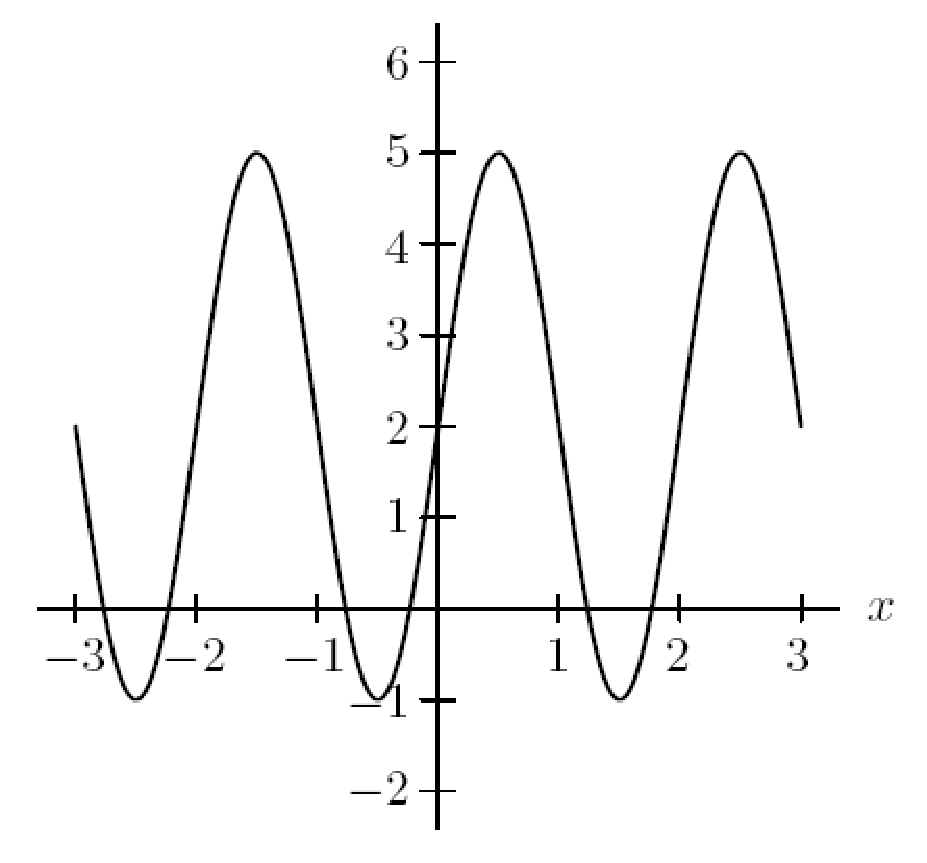
\includegraphics{SVC.01.05.010.ps}}

\begin{minipage}{0.4\columnwidth}
    \begin{enumerate}
        \item Amplitude = 2, Period = 2
        \item Amplitude = 2, Period = 3
        \item Amplitude = 2, Period = 1/2
        \item Amplitude = 3, Period = 2
        \item Amplitude = 3, Period = 1/2
    \end{enumerate}
\end{minipage}
\begin{minipage}{0.6\columnwidth}
    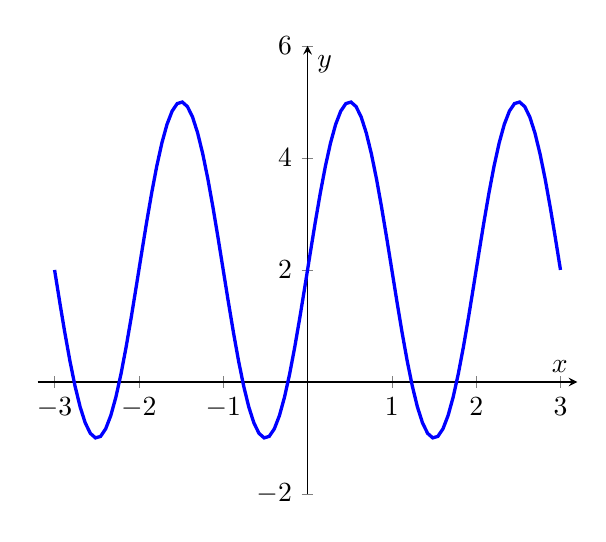
\begin{tikzpicture}
        \begin{axis}[axis lines=center, xlabel={$x$}, ylabel={$y$}, xmin=-3.2, xmax=3.2,
                ymin=-2, ymax=6]
                \addplot[color=blue, very thick,domain=-3:3, samples=100]
                {3*sin(pi*deg(x))+2};
            \end{axis}
    \end{tikzpicture}
\end{minipage}


% ConcepTests - to accompany Calculus 4th Edition, Hughes-Hallet et al. John Wiley \& Sons.
